\end{multicols}
\newpage
\begin{figure}[h]
\centering
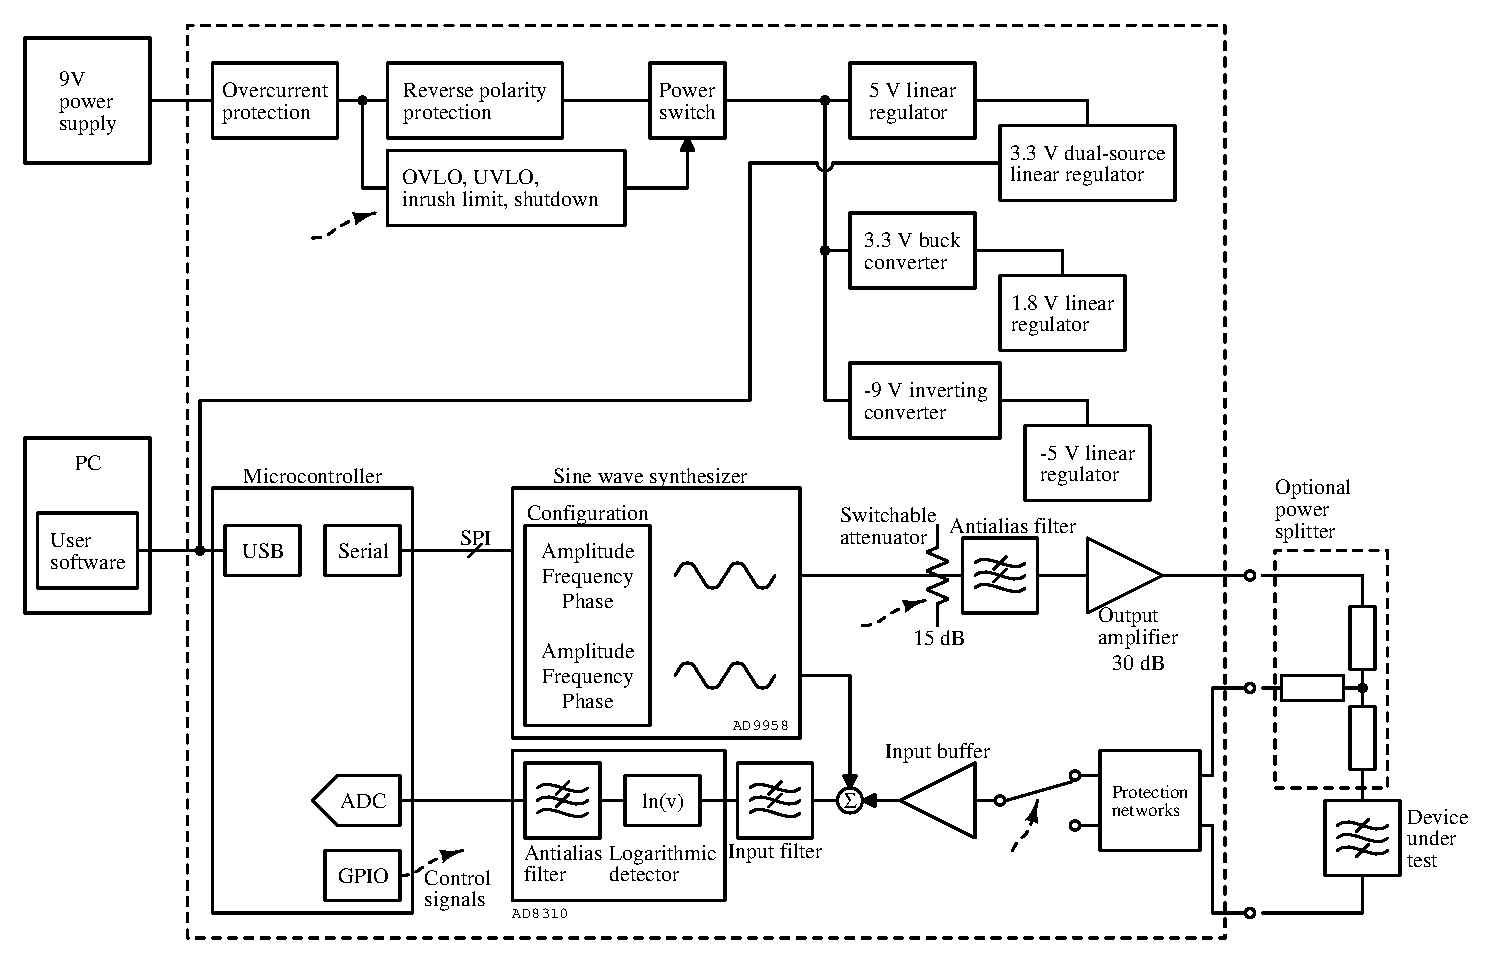
\includegraphics[width=6.5in]{blockdiagram}
\caption{Block diagram}
\label{fig:blockdiagram}
\end{figure}
\begin{multicols}{2}

\chapter{Theory of Operation}
\label{chap:too}

This section contains a decription of the operation of the gain/phase analyzer.
Explanations range from simple and broad to very specific.
It is expected that the reader has an understanding of the basics of
gain/phase analysis itself, which is explained in the \hyperref[chap:intro]{Introduction
chapter}.

Also, it will be beneficial to look at the main system schematics when reading
through this section. Small pieces of the schematic are excerpted when helpful
in explaining their function, but are not always shown.

\section{Block Description}

\schematicpage{1}{BlockDiagram}

The block diagram is shown in figure~\ref{fig:blockdiagram}. A microcontroller
drives the instrument, configuring a dual sine wave synthesizer via a serial
interface.  The first output passes through an optional, switchable attenuator,
allowing output amplitude to be configured beyond the practical amplitude range
of the synthesizer. The signal is then filtered to attenuate Nyquist aliasing,
and then amplified by 30~dB before being passed to the output.

Signals returning from the Device Under Test (DUT) pass through input protection
networks, then enter a double-throw RF switch allowing one of them to be
analyzed. An input buffer prevents signals from further circuitry from feeding
back out the input and affecting the DUT. A summing network combines the input
signal with the second output of the synthesizer, and the sum passes through an
input filter and into a logarithmic detector. The logarithmic detector outputs a
voltage corresponding to the signal amplitude in decibels, and this is further
filtered to allow slow sampling, and returns to the microcontroller via the
on-chip analog to digital converter.

A power supply system provides overcurrent protection, reverse polarity
protection, overvoltage lockout, undervoltage lockout, inrush limiting, and
microcontroller-driven shutdown (used in cases of USB suspend). It produces
regulated voltage rails of \Pos 9~V and \Neg 9~V (for the final output
amplifier stage), \Pos 5~V and \Neg 5~V (for general linear circuitry),
\Pos 3.3~V (for the synthesizer), \Pos 1.8~V (for the synthesizer),
and a second, weaker \Pos 3.3~V rail that can be powered by the USB port in
the absence of the main power input (for the microcontroller).

A USB interface connects to a computer, where software sends control commands to
the instrument and plots received data.
